\documentclass{whiteboard}
\begin{document}
\begin{frame}[plain,t]
\bbcover{OBI 2013 - Nível Júnior: Fase 1}{Saldo do Vovô}{Prof. Edson Alves}{Faculdade UnB Gama}

\end{frame}
\begin{frame}[plain,t]
\vspace*{\fill}

\bbtext{Vovô João tem uma banca de jornais; ele tem muitos clientes, e diariamente recebe muito dinheiro,
mas também faz muitos pagamentos para manter o seu estoque de jornais e revistas. Todo dia ele
vai ao banco realizar um depósito ou uma retirada de dinheiro. Em alguns dias, o saldo de sua conta
no banco fica negativo, mas Vovô João tem um acordo com o banco que garante que ele somente é
cobrado se o saldo for menor do que um valor pré-estabelecido.}


\vspace{0.2in}

\bbtext{Dada a movimentação diária da conta do banco do Vovô João, você deve escrever um programa que
calcule o menor saldo da conta, no período dado.}

\vspace*{\fill}
\end{frame}
\begin{frame}[plain,t]
\vspace*{\fill}

\bbbold{Entrada}

\vspace{0.2in}

\bbtext{A primeira linha da entrada contém dois números inteiros $N$ e $S$ que indicam respectivamente o
número de dias do período de interesse e o saldo da conta no início do período. Cada uma das $N$
linhas seguintes contém um número inteiro indicando a movimentação de um dia (valor positivo no
caso de depósito, valor negativo no caso de retirada). A movimentação é dada para um período de
$N$ dias consecutivos: a primeira das $N$ linhas corresponde ao primeiro dia do período de interesse,
a segunda linha corresponde ao segundo dia, e assim por diante.}

\vspace*{\fill}
\end{frame}
\begin{frame}[plain,t]
\vspace*{\fill}

\bbbold{Saída}

\vspace{0.2in}

\bbtext{Seu programa deve imprimir uma única linha, contendo um único número inteiro, o menor valor de
saldo da conta no período dado.}

\vspace{0.2in}

\bbbold{Restrições}
\vspace{-0.1in}

\bbtext{
\begin{itemize}
\item $1 \leq N \leq 30$
\item $-10^3 \leq S \leq 10^3$
\item $-10^3 \leq$ cada movimentação $\leq 10^3$
\end{itemize}
}

\vspace*{\fill}
\end{frame}
\begin{frame}[plain,t]
\begin{tikzpicture}
\node[draw,opacity=0] at (0, 0) {x};
\node[draw,opacity=0] at (14, 8) {x};

	\node[anchor=west] (header) at (0, 7.0) { \bbbold{Exemplo de entrada e saída} };

\end{tikzpicture}
\end{frame}
\begin{frame}[plain,t]
\begin{tikzpicture}
\node[draw,opacity=0] at (0, 0) {x};
\node[draw,opacity=0] at (14, 8) {x};

	\node[anchor=west] (header) at (0, 7.0) { \bbbold{Exemplo de entrada e saída} };


	\node[anchor=west] (line1) at (1.0, 6.0) { \bbtext{\texttt{6 -200}} };

\end{tikzpicture}
\end{frame}
\begin{frame}[plain,t]
\begin{tikzpicture}
\node[draw,opacity=0] at (0, 0) {x};
\node[draw,opacity=0] at (14, 8) {x};

	\node[anchor=west] (header) at (0, 7.0) { \bbbold{Exemplo de entrada e saída} };


	\node[anchor=west] (line1) at (1.0, 6.0) { \bbtext{\texttt{6 -200}} };


	\draw[->,color=BBViolet] (1.25, 5.0) to  (1.25, 5.75);

	\node[] (r) at (1.25, 4.75) { \footnotesize \bbcomment{\# de dias} };

\end{tikzpicture}
\end{frame}
\begin{frame}[plain,t]
\begin{tikzpicture}
\node[draw,opacity=0] at (0, 0) {x};
\node[draw,opacity=0] at (14, 8) {x};

	\node[anchor=west] (header) at (0, 7.0) { \bbbold{Exemplo de entrada e saída} };


	\node[anchor=west] (line1) at (1.0, 6.0) { \bbtext{\texttt{6 -200}} };


	\draw[->,color=BBViolet] (2.03, 5.0) to  (2.03, 5.75);

	\node[] (r) at (2.03, 4.75) { \footnotesize \bbcomment{saldo inicial} };



\end{tikzpicture}
\end{frame}
\begin{frame}[plain,t]
\begin{tikzpicture}
\node[draw,opacity=0] at (0, 0) {x};
\node[draw,opacity=0] at (14, 8) {x};

	\node[anchor=west] (header) at (0, 7.0) { \bbbold{Exemplo de entrada e saída} };


	\node[anchor=west] (line1) at (1.0, 6.0) { \bbtext{\texttt{6 -200}} };








	\node[] (granpa) at (11.0, 4.5) { \includegraphics[scale=0.3]{figs/grandfather.png} };

	\node[] (cash) at (11.0, 1.75) { \Large \bbtext{-200} };

	\node[] (answer) at (11.0, 1.0) { \large \bboutput{-200} };

\end{tikzpicture}
\end{frame}
\begin{frame}[plain,t]
\begin{tikzpicture}
\node[draw,opacity=0] at (0, 0) {x};
\node[draw,opacity=0] at (14, 8) {x};

	\node[anchor=west] (header) at (0, 7.0) { \bbbold{Exemplo de entrada e saída} };


	\node[anchor=west] (line1) at (1.0, 6.0) { \bbtext{\texttt{6 -200}} };








	\node[] (granpa) at (11.0, 4.5) { \includegraphics[scale=0.3]{figs/grandfather.png} };

	\node[] (cash) at (11.0, 1.75) { \Large \bbtext{-200} };

	\node[] (answer) at (11.0, 1.0) { \large \bboutput{-200} };


	\node[anchor=west] (line2) at (1.0, 5.5) { \bbtext{\texttt{-100}} };

\end{tikzpicture}
\end{frame}
\begin{frame}[plain,t]
\begin{tikzpicture}
\node[draw,opacity=0] at (0, 0) {x};
\node[draw,opacity=0] at (14, 8) {x};

	\node[anchor=west] (header) at (0, 7.0) { \bbbold{Exemplo de entrada e saída} };


	\node[anchor=west] (line1) at (1.0, 6.0) { \bbtext{\texttt{6 -200}} };


	\draw[->,color=BBViolet] (3.0, 5.5) to  (2.25, 5.5);

	\node[anchor=west] (r) at (3.1, 5.5) { \footnotesize \bbcomment{retirada no dia $1$} };





	\node[] (granpa) at (11.0, 4.5) { \includegraphics[scale=0.3]{figs/grandfather.png} };

	\node[] (cash) at (11.0, 1.75) { \Large \bbtext{-200} };

	\node[] (answer) at (11.0, 1.0) { \large \bboutput{-200} };


	\node[anchor=west] (line2) at (1.0, 5.5) { \bbtext{\texttt{-100}} };


\end{tikzpicture}
\end{frame}
\begin{frame}[plain,t]
\begin{tikzpicture}
\node[draw,opacity=0] at (0, 0) {x};
\node[draw,opacity=0] at (14, 8) {x};

	\node[anchor=west] (header) at (0, 7.0) { \bbbold{Exemplo de entrada e saída} };


	\node[anchor=west] (line1) at (1.0, 6.0) { \bbtext{\texttt{6 -200}} };








	\node[] (granpa) at (11.0, 4.5) { \includegraphics[scale=0.3]{figs/grandfather.png} };

	\node[] (cash) at (11.0, 1.75) { \Large \bbtext{-300} };

	\node[] (answer) at (11.0, 1.0) { \large \bboutput{-200} };


	\node[anchor=west] (line2) at (1.0, 5.5) { \bbtext{\texttt{-100}} };



\end{tikzpicture}
\end{frame}
\begin{frame}[plain,t]
\begin{tikzpicture}
\node[draw,opacity=0] at (0, 0) {x};
\node[draw,opacity=0] at (14, 8) {x};

	\node[anchor=west] (header) at (0, 7.0) { \bbbold{Exemplo de entrada e saída} };


	\node[anchor=west] (line1) at (1.0, 6.0) { \bbtext{\texttt{6 -200}} };








	\node[] (granpa) at (11.0, 4.5) { \includegraphics[scale=0.3]{figs/grandfather.png} };

	\node[] (cash) at (11.0, 1.75) { \Large \bbtext{-300} };

	\node[] (answer) at (11.0, 1.0) { \large \bboutput{-300} };


	\node[anchor=west] (line2) at (1.0, 5.5) { \bbtext{\texttt{-100}} };




\end{tikzpicture}
\end{frame}
\begin{frame}[plain,t]
\begin{tikzpicture}
\node[draw,opacity=0] at (0, 0) {x};
\node[draw,opacity=0] at (14, 8) {x};

	\node[anchor=west] (header) at (0, 7.0) { \bbbold{Exemplo de entrada e saída} };


	\node[anchor=west] (line1) at (1.0, 6.0) { \bbtext{\texttt{6 -200}} };








	\node[] (granpa) at (11.0, 4.5) { \includegraphics[scale=0.3]{figs/grandfather.png} };

	\node[] (cash) at (11.0, 1.75) { \Large \bbtext{-300} };

	\node[] (answer) at (11.0, 1.0) { \large \bboutput{-300} };


	\node[anchor=west] (line2) at (1.0, 5.5) { \bbtext{\texttt{-100}} };





	\node[anchor=west] (line3) at (1.0, 5.0) { \bbtext{\texttt{1000}} };

\end{tikzpicture}
\end{frame}
\begin{frame}[plain,t]
\begin{tikzpicture}
\node[draw,opacity=0] at (0, 0) {x};
\node[draw,opacity=0] at (14, 8) {x};

	\node[anchor=west] (header) at (0, 7.0) { \bbbold{Exemplo de entrada e saída} };


	\node[anchor=west] (line1) at (1.0, 6.0) { \bbtext{\texttt{6 -200}} };


	\draw[->,color=BBViolet] (3.0, 5.0) to  (2.25, 5.0);

	\node[anchor=west] (r) at (3.1, 5.0) { \footnotesize \bbcomment{depósito no dia $2$} };





	\node[] (granpa) at (11.0, 4.5) { \includegraphics[scale=0.3]{figs/grandfather.png} };

	\node[] (cash) at (11.0, 1.75) { \Large \bbtext{-300} };

	\node[] (answer) at (11.0, 1.0) { \large \bboutput{-300} };


	\node[anchor=west] (line2) at (1.0, 5.5) { \bbtext{\texttt{-100}} };





	\node[anchor=west] (line3) at (1.0, 5.0) { \bbtext{\texttt{1000}} };



\end{tikzpicture}
\end{frame}
\begin{frame}[plain,t]
\begin{tikzpicture}
\node[draw,opacity=0] at (0, 0) {x};
\node[draw,opacity=0] at (14, 8) {x};

	\node[anchor=west] (header) at (0, 7.0) { \bbbold{Exemplo de entrada e saída} };


	\node[anchor=west] (line1) at (1.0, 6.0) { \bbtext{\texttt{6 -200}} };








	\node[] (granpa) at (11.0, 4.5) { \includegraphics[scale=0.3]{figs/grandfather.png} };

	\node[] (cash) at (11.0, 1.75) { \Large \bbtext{700} };

	\node[] (answer) at (11.0, 1.0) { \large \bboutput{-300} };


	\node[anchor=west] (line2) at (1.0, 5.5) { \bbtext{\texttt{-100}} };





	\node[anchor=west] (line3) at (1.0, 5.0) { \bbtext{\texttt{1000}} };





\end{tikzpicture}
\end{frame}
\begin{frame}[plain,t]
\begin{tikzpicture}
\node[draw,opacity=0] at (0, 0) {x};
\node[draw,opacity=0] at (14, 8) {x};

	\node[anchor=west] (header) at (0, 7.0) { \bbbold{Exemplo de entrada e saída} };


	\node[anchor=west] (line1) at (1.0, 6.0) { \bbtext{\texttt{6 -200}} };








	\node[] (granpa) at (11.0, 4.5) { \includegraphics[scale=0.3]{figs/grandfather.png} };

	\node[] (cash) at (11.0, 1.75) { \Large \bbtext{700} };

	\node[] (answer) at (11.0, 1.0) { \large \bboutput{-300} };


	\node[anchor=west] (line2) at (1.0, 5.5) { \bbtext{\texttt{-100}} };





	\node[anchor=west] (line3) at (1.0, 5.0) { \bbtext{\texttt{1000}} };






	\node[anchor=west] (line4) at (1.0, 4.5) { \bbtext{\texttt{-2000}} };

\end{tikzpicture}
\end{frame}
\begin{frame}[plain,t]
\begin{tikzpicture}
\node[draw,opacity=0] at (0, 0) {x};
\node[draw,opacity=0] at (14, 8) {x};

	\node[anchor=west] (header) at (0, 7.0) { \bbbold{Exemplo de entrada e saída} };


	\node[anchor=west] (line1) at (1.0, 6.0) { \bbtext{\texttt{6 -200}} };


	\draw[->,color=BBViolet] (3.0, 4.5) to  (2.25, 4.5);

	\node[anchor=west] (r) at (3.1, 4.5) { \footnotesize \bbcomment{retirada no dia $3$} };





	\node[] (granpa) at (11.0, 4.5) { \includegraphics[scale=0.3]{figs/grandfather.png} };

	\node[] (cash) at (11.0, 1.75) { \Large \bbtext{700} };

	\node[] (answer) at (11.0, 1.0) { \large \bboutput{-300} };


	\node[anchor=west] (line2) at (1.0, 5.5) { \bbtext{\texttt{-100}} };





	\node[anchor=west] (line3) at (1.0, 5.0) { \bbtext{\texttt{1000}} };






	\node[anchor=west] (line4) at (1.0, 4.5) { \bbtext{\texttt{-2000}} };



\end{tikzpicture}
\end{frame}
\begin{frame}[plain,t]
\begin{tikzpicture}
\node[draw,opacity=0] at (0, 0) {x};
\node[draw,opacity=0] at (14, 8) {x};

	\node[anchor=west] (header) at (0, 7.0) { \bbbold{Exemplo de entrada e saída} };


	\node[anchor=west] (line1) at (1.0, 6.0) { \bbtext{\texttt{6 -200}} };








	\node[] (granpa) at (11.0, 4.5) { \includegraphics[scale=0.3]{figs/grandfather.png} };

	\node[] (cash) at (11.0, 1.75) { \Large \bbtext{-1300} };

	\node[] (answer) at (11.0, 1.0) { \large \bboutput{-300} };


	\node[anchor=west] (line2) at (1.0, 5.5) { \bbtext{\texttt{-100}} };





	\node[anchor=west] (line3) at (1.0, 5.0) { \bbtext{\texttt{1000}} };






	\node[anchor=west] (line4) at (1.0, 4.5) { \bbtext{\texttt{-2000}} };




\end{tikzpicture}
\end{frame}
\begin{frame}[plain,t]
\begin{tikzpicture}
\node[draw,opacity=0] at (0, 0) {x};
\node[draw,opacity=0] at (14, 8) {x};

	\node[anchor=west] (header) at (0, 7.0) { \bbbold{Exemplo de entrada e saída} };


	\node[anchor=west] (line1) at (1.0, 6.0) { \bbtext{\texttt{6 -200}} };








	\node[] (granpa) at (11.0, 4.5) { \includegraphics[scale=0.3]{figs/grandfather.png} };

	\node[] (cash) at (11.0, 1.75) { \Large \bbtext{-1300} };

	\node[] (answer) at (11.0, 1.0) { \Large \bboutput{-1300} };


	\node[anchor=west] (line2) at (1.0, 5.5) { \bbtext{\texttt{-100}} };





	\node[anchor=west] (line3) at (1.0, 5.0) { \bbtext{\texttt{1000}} };






	\node[anchor=west] (line4) at (1.0, 4.5) { \bbtext{\texttt{-2000}} };





\end{tikzpicture}
\end{frame}
\begin{frame}[plain,t]
\begin{tikzpicture}
\node[draw,opacity=0] at (0, 0) {x};
\node[draw,opacity=0] at (14, 8) {x};

	\node[anchor=west] (header) at (0, 7.0) { \bbbold{Exemplo de entrada e saída} };


	\node[anchor=west] (line1) at (1.0, 6.0) { \bbtext{\texttt{6 -200}} };








	\node[] (granpa) at (11.0, 4.5) { \includegraphics[scale=0.3]{figs/grandfather.png} };

	\node[] (cash) at (11.0, 1.75) { \Large \bbtext{-1300} };

	\node[] (answer) at (11.0, 1.0) { \Large \bboutput{-1300} };


	\node[anchor=west] (line2) at (1.0, 5.5) { \bbtext{\texttt{-100}} };





	\node[anchor=west] (line3) at (1.0, 5.0) { \bbtext{\texttt{1000}} };






	\node[anchor=west] (line4) at (1.0, 4.5) { \bbtext{\texttt{-2000}} };






	\node[anchor=west] (line5) at (1.0, 4.0) { \bbtext{\texttt{100}} };

\end{tikzpicture}
\end{frame}
\begin{frame}[plain,t]
\begin{tikzpicture}
\node[draw,opacity=0] at (0, 0) {x};
\node[draw,opacity=0] at (14, 8) {x};

	\node[anchor=west] (header) at (0, 7.0) { \bbbold{Exemplo de entrada e saída} };


	\node[anchor=west] (line1) at (1.0, 6.0) { \bbtext{\texttt{6 -200}} };


	\draw[->,color=BBViolet] (3.0, 4.0) to  (2.25, 4.0);

	\node[anchor=west] (r) at (3.1, 4.0) { \footnotesize \bbcomment{depósito no dia $4$} };





	\node[] (granpa) at (11.0, 4.5) { \includegraphics[scale=0.3]{figs/grandfather.png} };

	\node[] (cash) at (11.0, 1.75) { \Large \bbtext{-1300} };

	\node[] (answer) at (11.0, 1.0) { \Large \bboutput{-1300} };


	\node[anchor=west] (line2) at (1.0, 5.5) { \bbtext{\texttt{-100}} };





	\node[anchor=west] (line3) at (1.0, 5.0) { \bbtext{\texttt{1000}} };






	\node[anchor=west] (line4) at (1.0, 4.5) { \bbtext{\texttt{-2000}} };






	\node[anchor=west] (line5) at (1.0, 4.0) { \bbtext{\texttt{100}} };



\end{tikzpicture}
\end{frame}
\begin{frame}[plain,t]
\begin{tikzpicture}
\node[draw,opacity=0] at (0, 0) {x};
\node[draw,opacity=0] at (14, 8) {x};

	\node[anchor=west] (header) at (0, 7.0) { \bbbold{Exemplo de entrada e saída} };


	\node[anchor=west] (line1) at (1.0, 6.0) { \bbtext{\texttt{6 -200}} };








	\node[] (granpa) at (11.0, 4.5) { \includegraphics[scale=0.3]{figs/grandfather.png} };

	\node[] (cash) at (11.0, 1.75) { \Large \bbtext{-1200} };

	\node[] (answer) at (11.0, 1.0) { \Large \bboutput{-1300} };


	\node[anchor=west] (line2) at (1.0, 5.5) { \bbtext{\texttt{-100}} };





	\node[anchor=west] (line3) at (1.0, 5.0) { \bbtext{\texttt{1000}} };






	\node[anchor=west] (line4) at (1.0, 4.5) { \bbtext{\texttt{-2000}} };






	\node[anchor=west] (line5) at (1.0, 4.0) { \bbtext{\texttt{100}} };





\end{tikzpicture}
\end{frame}
\begin{frame}[plain,t]
\begin{tikzpicture}
\node[draw,opacity=0] at (0, 0) {x};
\node[draw,opacity=0] at (14, 8) {x};

	\node[anchor=west] (header) at (0, 7.0) { \bbbold{Exemplo de entrada e saída} };


	\node[anchor=west] (line1) at (1.0, 6.0) { \bbtext{\texttt{6 -200}} };








	\node[] (granpa) at (11.0, 4.5) { \includegraphics[scale=0.3]{figs/grandfather.png} };

	\node[] (cash) at (11.0, 1.75) { \Large \bbtext{-1200} };

	\node[] (answer) at (11.0, 1.0) { \Large \bboutput{-1300} };


	\node[anchor=west] (line2) at (1.0, 5.5) { \bbtext{\texttt{-100}} };





	\node[anchor=west] (line3) at (1.0, 5.0) { \bbtext{\texttt{1000}} };






	\node[anchor=west] (line4) at (1.0, 4.5) { \bbtext{\texttt{-2000}} };






	\node[anchor=west] (line5) at (1.0, 4.0) { \bbtext{\texttt{100}} };






	\node[anchor=west] (line6) at (1.0, 3.5) { \bbtext{\texttt{-50}} };

\end{tikzpicture}
\end{frame}
\begin{frame}[plain,t]
\begin{tikzpicture}
\node[draw,opacity=0] at (0, 0) {x};
\node[draw,opacity=0] at (14, 8) {x};

	\node[anchor=west] (header) at (0, 7.0) { \bbbold{Exemplo de entrada e saída} };


	\node[anchor=west] (line1) at (1.0, 6.0) { \bbtext{\texttt{6 -200}} };


	\draw[->,color=BBViolet] (3.0, 3.5) to  (2.25, 3.5);

	\node[anchor=west] (r) at (3.1, 3.5) { \footnotesize \bbcomment{retirada no dia $5$} };





	\node[] (granpa) at (11.0, 4.5) { \includegraphics[scale=0.3]{figs/grandfather.png} };

	\node[] (cash) at (11.0, 1.75) { \Large \bbtext{-1200} };

	\node[] (answer) at (11.0, 1.0) { \Large \bboutput{-1300} };


	\node[anchor=west] (line2) at (1.0, 5.5) { \bbtext{\texttt{-100}} };





	\node[anchor=west] (line3) at (1.0, 5.0) { \bbtext{\texttt{1000}} };






	\node[anchor=west] (line4) at (1.0, 4.5) { \bbtext{\texttt{-2000}} };






	\node[anchor=west] (line5) at (1.0, 4.0) { \bbtext{\texttt{100}} };






	\node[anchor=west] (line6) at (1.0, 3.5) { \bbtext{\texttt{-50}} };



\end{tikzpicture}
\end{frame}
\begin{frame}[plain,t]
\begin{tikzpicture}
\node[draw,opacity=0] at (0, 0) {x};
\node[draw,opacity=0] at (14, 8) {x};

	\node[anchor=west] (header) at (0, 7.0) { \bbbold{Exemplo de entrada e saída} };


	\node[anchor=west] (line1) at (1.0, 6.0) { \bbtext{\texttt{6 -200}} };








	\node[] (granpa) at (11.0, 4.5) { \includegraphics[scale=0.3]{figs/grandfather.png} };

	\node[] (cash) at (11.0, 1.75) { \Large \bbtext{-1250} };

	\node[] (answer) at (11.0, 1.0) { \Large \bboutput{-1300} };


	\node[anchor=west] (line2) at (1.0, 5.5) { \bbtext{\texttt{-100}} };





	\node[anchor=west] (line3) at (1.0, 5.0) { \bbtext{\texttt{1000}} };






	\node[anchor=west] (line4) at (1.0, 4.5) { \bbtext{\texttt{-2000}} };






	\node[anchor=west] (line5) at (1.0, 4.0) { \bbtext{\texttt{100}} };






	\node[anchor=west] (line6) at (1.0, 3.5) { \bbtext{\texttt{-50}} };





\end{tikzpicture}
\end{frame}
\begin{frame}[plain,t]
\begin{tikzpicture}
\node[draw,opacity=0] at (0, 0) {x};
\node[draw,opacity=0] at (14, 8) {x};

	\node[anchor=west] (header) at (0, 7.0) { \bbbold{Exemplo de entrada e saída} };


	\node[anchor=west] (line1) at (1.0, 6.0) { \bbtext{\texttt{6 -200}} };








	\node[] (granpa) at (11.0, 4.5) { \includegraphics[scale=0.3]{figs/grandfather.png} };

	\node[] (cash) at (11.0, 1.75) { \Large \bbtext{-1250} };

	\node[] (answer) at (11.0, 1.0) { \Large \bboutput{-1300} };


	\node[anchor=west] (line2) at (1.0, 5.5) { \bbtext{\texttt{-100}} };





	\node[anchor=west] (line3) at (1.0, 5.0) { \bbtext{\texttt{1000}} };






	\node[anchor=west] (line4) at (1.0, 4.5) { \bbtext{\texttt{-2000}} };






	\node[anchor=west] (line5) at (1.0, 4.0) { \bbtext{\texttt{100}} };






	\node[anchor=west] (line6) at (1.0, 3.5) { \bbtext{\texttt{-50}} };






	\node[anchor=west] (line7) at (1.0, 3.0) { \bbtext{\texttt{2000}} };

\end{tikzpicture}
\end{frame}
\begin{frame}[plain,t]
\begin{tikzpicture}
\node[draw,opacity=0] at (0, 0) {x};
\node[draw,opacity=0] at (14, 8) {x};

	\node[anchor=west] (header) at (0, 7.0) { \bbbold{Exemplo de entrada e saída} };


	\node[anchor=west] (line1) at (1.0, 6.0) { \bbtext{\texttt{6 -200}} };


	\draw[->,color=BBViolet] (3.0, 3.0) to  (2.25, 3.0);

	\node[anchor=west] (r) at (3.1, 3.0) { \footnotesize \bbcomment{depósito no dia $6$} };





	\node[] (granpa) at (11.0, 4.5) { \includegraphics[scale=0.3]{figs/grandfather.png} };

	\node[] (cash) at (11.0, 1.75) { \Large \bbtext{-1250} };

	\node[] (answer) at (11.0, 1.0) { \Large \bboutput{-1300} };


	\node[anchor=west] (line2) at (1.0, 5.5) { \bbtext{\texttt{-100}} };





	\node[anchor=west] (line3) at (1.0, 5.0) { \bbtext{\texttt{1000}} };






	\node[anchor=west] (line4) at (1.0, 4.5) { \bbtext{\texttt{-2000}} };






	\node[anchor=west] (line5) at (1.0, 4.0) { \bbtext{\texttt{100}} };






	\node[anchor=west] (line6) at (1.0, 3.5) { \bbtext{\texttt{-50}} };






	\node[anchor=west] (line7) at (1.0, 3.0) { \bbtext{\texttt{2000}} };



\end{tikzpicture}
\end{frame}
\begin{frame}[plain,t]
\begin{tikzpicture}
\node[draw,opacity=0] at (0, 0) {x};
\node[draw,opacity=0] at (14, 8) {x};

	\node[anchor=west] (header) at (0, 7.0) { \bbbold{Exemplo de entrada e saída} };


	\node[anchor=west] (line1) at (1.0, 6.0) { \bbtext{\texttt{6 -200}} };








	\node[] (granpa) at (11.0, 4.5) { \includegraphics[scale=0.3]{figs/grandfather.png} };

	\node[] (cash) at (11.0, 1.75) { \Large \bbtext{800} };

	\node[] (answer) at (11.0, 1.0) { \Large \bboutput{-1300} };


	\node[anchor=west] (line2) at (1.0, 5.5) { \bbtext{\texttt{-100}} };





	\node[anchor=west] (line3) at (1.0, 5.0) { \bbtext{\texttt{1000}} };






	\node[anchor=west] (line4) at (1.0, 4.5) { \bbtext{\texttt{-2000}} };






	\node[anchor=west] (line5) at (1.0, 4.0) { \bbtext{\texttt{100}} };






	\node[anchor=west] (line6) at (1.0, 3.5) { \bbtext{\texttt{-50}} };






	\node[anchor=west] (line7) at (1.0, 3.0) { \bbtext{\texttt{2000}} };





\end{tikzpicture}
\end{frame}
\begin{frame}[plain,t]
\begin{tikzpicture}
\node[draw,opacity=0] at (0, 0) {x};
\node[draw,opacity=0] at (14, 8) {x};

	\node[anchor=west] (title) at (0.0, 7.0) { \Large \bbbold{Solução} };

\end{tikzpicture}
\end{frame}
\begin{frame}[plain,t]
\begin{tikzpicture}
\node[draw,opacity=0] at (0, 0) {x};
\node[draw,opacity=0] at (14, 8) {x};

	\node[anchor=west] (title) at (0.0, 7.0) { \Large \bbbold{Solução} };


	\node[anchor=west] (a) at (1.0, 6.0) { $\star$ \bbtext{O problema consiste em simular as ações do vovô a cada dia} };

\end{tikzpicture}
\end{frame}
\begin{frame}[plain,t]
\begin{tikzpicture}
\node[draw,opacity=0] at (0, 0) {x};
\node[draw,opacity=0] at (14, 8) {x};

	\node[anchor=west] (title) at (0.0, 7.0) { \Large \bbbold{Solução} };


	\node[anchor=west] (a) at (1.0, 6.0) { $\star$ \bbtext{O problema consiste em simular as ações do vovô a cada dia} };


	\node[anchor=west] (b) at (1.0, 5.0) { $\star$ \bbtext{Devem ser mantidas duas variáveis: o saldo atual e o menor saldo da série histórica} };

\end{tikzpicture}
\end{frame}
\begin{frame}[plain,t]
\begin{tikzpicture}
\node[draw,opacity=0] at (0, 0) {x};
\node[draw,opacity=0] at (14, 8) {x};

	\node[anchor=west] (title) at (0.0, 7.0) { \Large \bbbold{Solução} };


	\node[anchor=west] (a) at (1.0, 6.0) { $\star$ \bbtext{O problema consiste em simular as ações do vovô a cada dia} };


	\node[anchor=west] (b) at (1.0, 5.0) { $\star$ \bbtext{Devem ser mantidas duas variáveis: o saldo atual e o menor saldo da série histórica} };


	\node[anchor=west] (c) at (1.0, 4.0) { $\star$ \bbtext{É necessário um laço de se repita $N$ vezes para ler a entrada} };

\end{tikzpicture}
\end{frame}
\begin{frame}[plain,t]
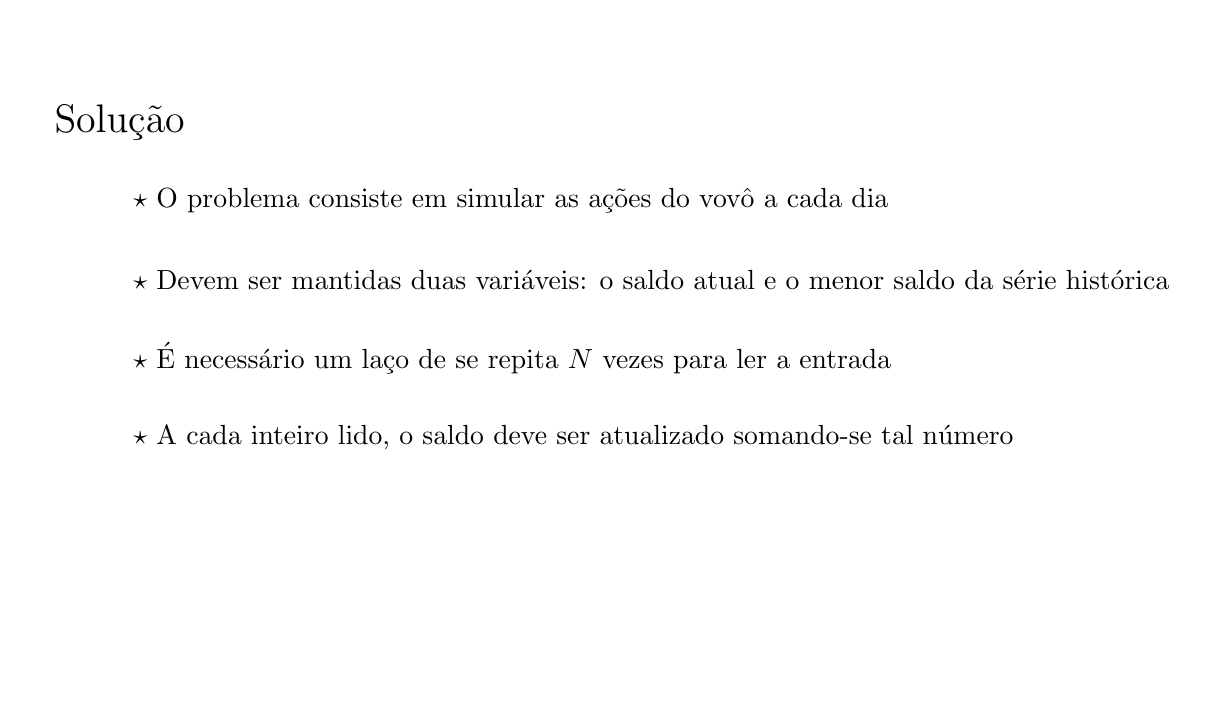
\begin{tikzpicture}
\node[draw,opacity=0] at (0, 0) {x};
\node[draw,opacity=0] at (14, 8) {x};

	\node[anchor=west] (title) at (0.0, 7.0) { \Large \bbbold{Solução} };


	\node[anchor=west] (a) at (1.0, 6.0) { $\star$ \bbtext{O problema consiste em simular as ações do vovô a cada dia} };


	\node[anchor=west] (b) at (1.0, 5.0) { $\star$ \bbtext{Devem ser mantidas duas variáveis: o saldo atual e o menor saldo da série histórica} };


	\node[anchor=west] (c) at (1.0, 4.0) { $\star$ \bbtext{É necessário um laço de se repita $N$ vezes para ler a entrada} };


	\node[anchor=west] (d) at (1.0, 3.0) { $\star$ \bbtext{A cada inteiro lido, o saldo deve ser atualizado somando-se tal número} };

\end{tikzpicture}
\end{frame}
\begin{frame}[plain,t]
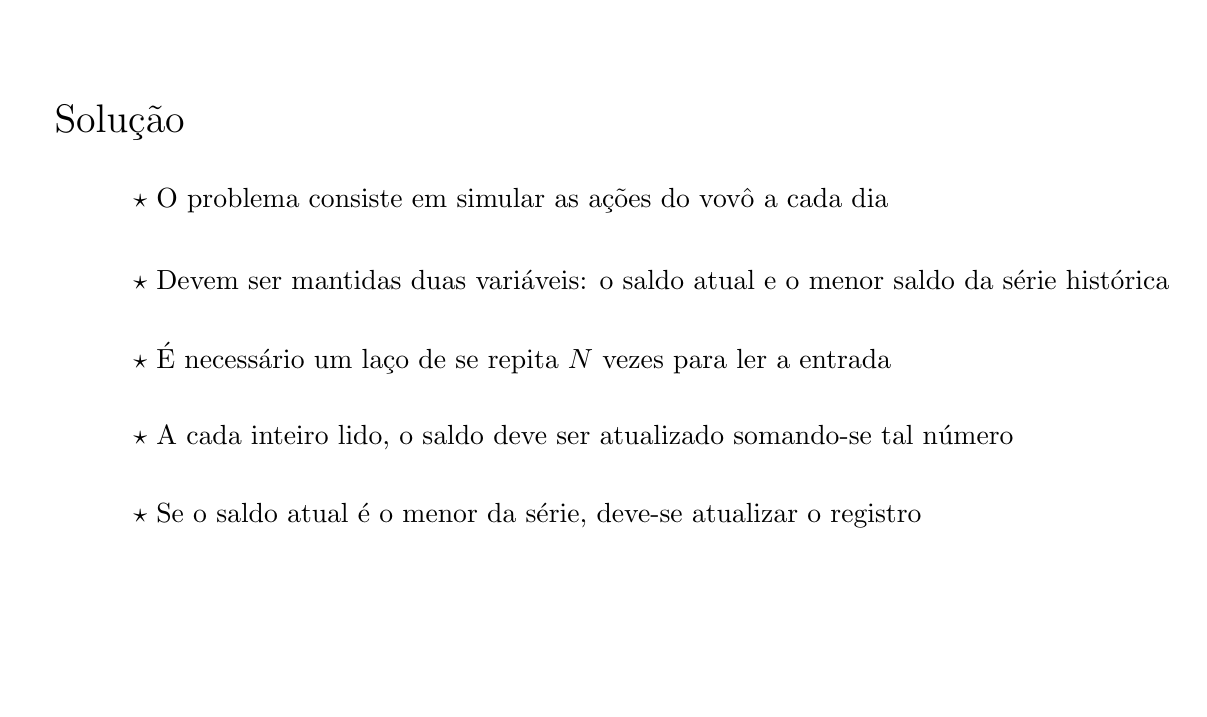
\begin{tikzpicture}
\node[draw,opacity=0] at (0, 0) {x};
\node[draw,opacity=0] at (14, 8) {x};

	\node[anchor=west] (title) at (0.0, 7.0) { \Large \bbbold{Solução} };


	\node[anchor=west] (a) at (1.0, 6.0) { $\star$ \bbtext{O problema consiste em simular as ações do vovô a cada dia} };


	\node[anchor=west] (b) at (1.0, 5.0) { $\star$ \bbtext{Devem ser mantidas duas variáveis: o saldo atual e o menor saldo da série histórica} };


	\node[anchor=west] (c) at (1.0, 4.0) { $\star$ \bbtext{É necessário um laço de se repita $N$ vezes para ler a entrada} };


	\node[anchor=west] (d) at (1.0, 3.0) { $\star$ \bbtext{A cada inteiro lido, o saldo deve ser atualizado somando-se tal número} };


	\node[anchor=west] (e) at (1.0, 2.0) { $\star$ \bbtext{Se o saldo atual é o menor da série, deve-se atualizar o registro} };

\end{tikzpicture}
\end{frame}
\begin{frame}[plain,t]
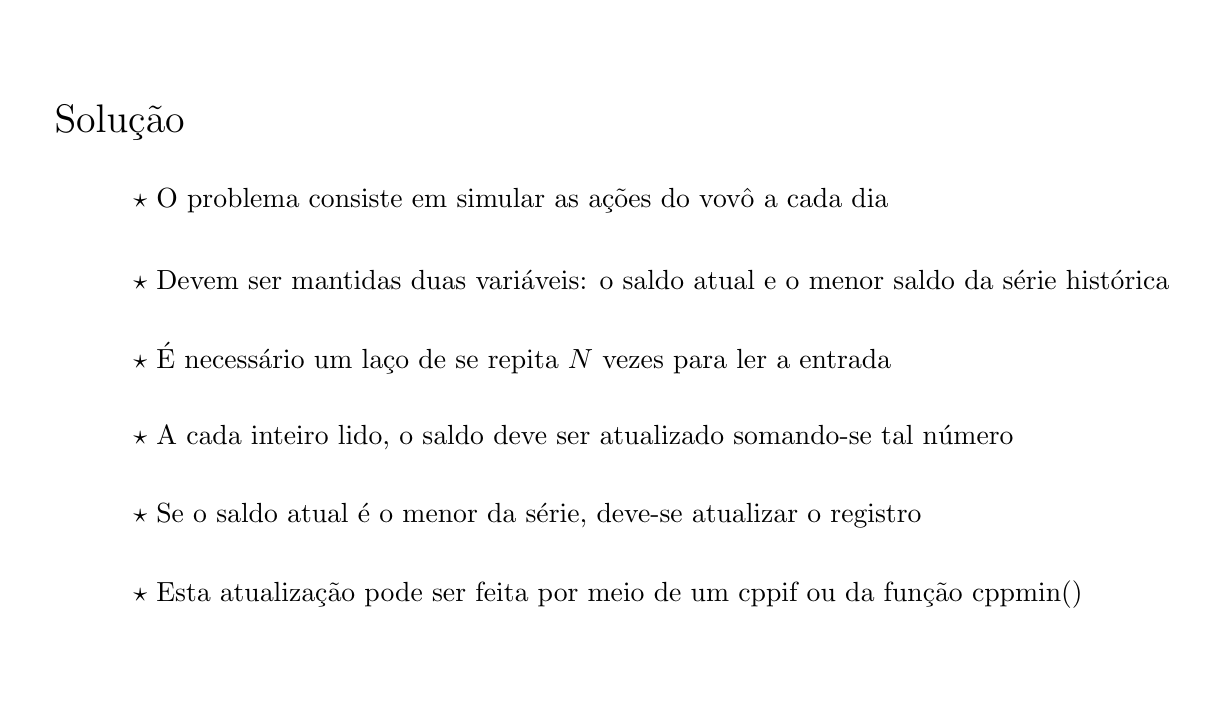
\begin{tikzpicture}
\node[draw,opacity=0] at (0, 0) {x};
\node[draw,opacity=0] at (14, 8) {x};

	\node[anchor=west] (title) at (0.0, 7.0) { \Large \bbbold{Solução} };


	\node[anchor=west] (a) at (1.0, 6.0) { $\star$ \bbtext{O problema consiste em simular as ações do vovô a cada dia} };


	\node[anchor=west] (b) at (1.0, 5.0) { $\star$ \bbtext{Devem ser mantidas duas variáveis: o saldo atual e o menor saldo da série histórica} };


	\node[anchor=west] (c) at (1.0, 4.0) { $\star$ \bbtext{É necessário um laço de se repita $N$ vezes para ler a entrada} };


	\node[anchor=west] (d) at (1.0, 3.0) { $\star$ \bbtext{A cada inteiro lido, o saldo deve ser atualizado somando-se tal número} };


	\node[anchor=west] (e) at (1.0, 2.0) { $\star$ \bbtext{Se o saldo atual é o menor da série, deve-se atualizar o registro} };


	\node[anchor=west] (f) at (1.0, 1.0) { $\star$ \bbtext{Esta atualização pode ser feita por meio de um \mintinline{cpp}{if} ou da função \mintinline{cpp}{min()}} };

\end{tikzpicture}
\end{frame}
\begin{frame}[plain,t]
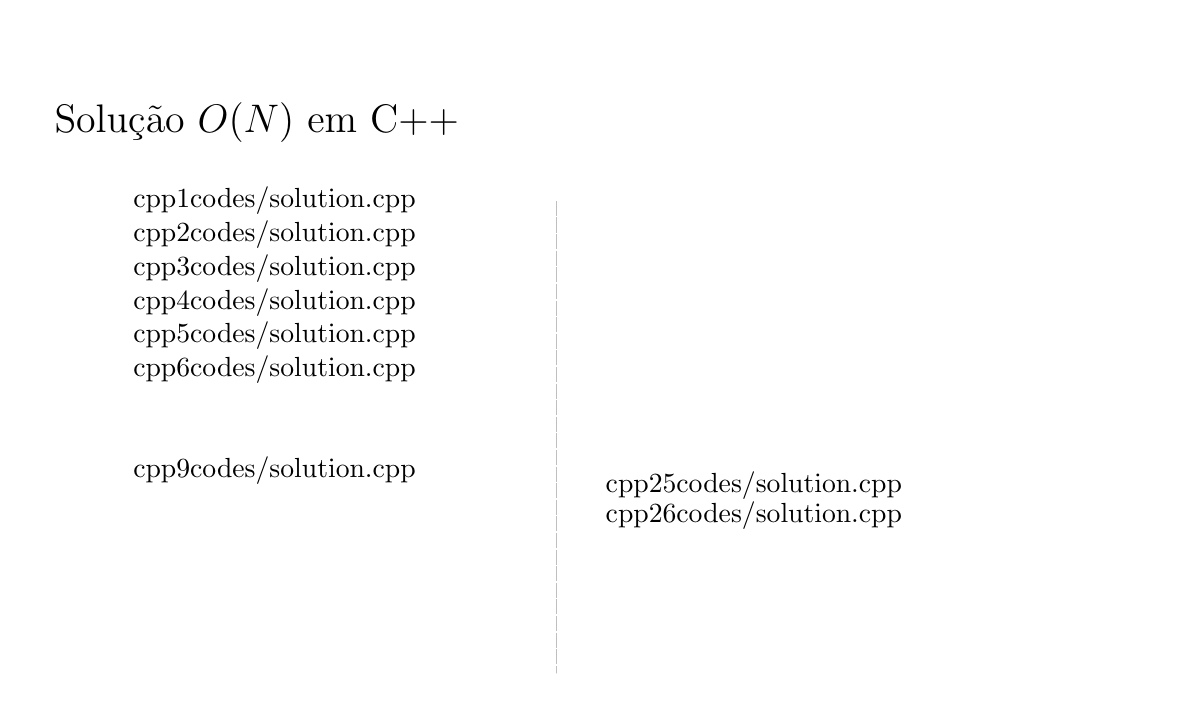
\begin{tikzpicture}
\node[draw,opacity=0] at (0, 0) {x};
\node[draw,opacity=0] at (14, 8) {x};

	\node[anchor=west] (title) at (0.0, 7.0) { \Large \bbbold{Solução $O(N)$ em C++} };

	\node[anchor=west] (line1) at (1.0, 6.0) { \inputline{cpp}{1}{codes/solution.cpp} };

	\node[anchor=west] (line2) at (1.0, 5.57) { \inputline{cpp}{2}{codes/solution.cpp} };

	\node[anchor=west] (line3) at (1.0, 5.14) { \inputline{cpp}{3}{codes/solution.cpp} };

	\node[anchor=west] (line4) at (1.0, 4.71) { \inputline{cpp}{4}{codes/solution.cpp} };

	\node[anchor=west] (line5) at (1.0, 4.29) { \inputline{cpp}{5}{codes/solution.cpp} };

	\node[anchor=west] (line6) at (1.0, 3.86) { \inputline{cpp}{6}{codes/solution.cpp} };



	\node[anchor=west] (line9) at (1.0, 2.57) { \inputline{cpp}{9}{codes/solution.cpp} };















	\node[anchor=west] (line25) at (7.0, 2.39) { \inputline{cpp}{25}{codes/solution.cpp} };

	\node[anchor=west] (line26) at (7.0, 2.0) { \inputline{cpp}{26}{codes/solution.cpp} };

	\draw[color=gray!50,dashed] (6.5, 6) -- (6.5, 0) -- cycle;


\end{tikzpicture}
\end{frame}
\begin{frame}[plain,t]
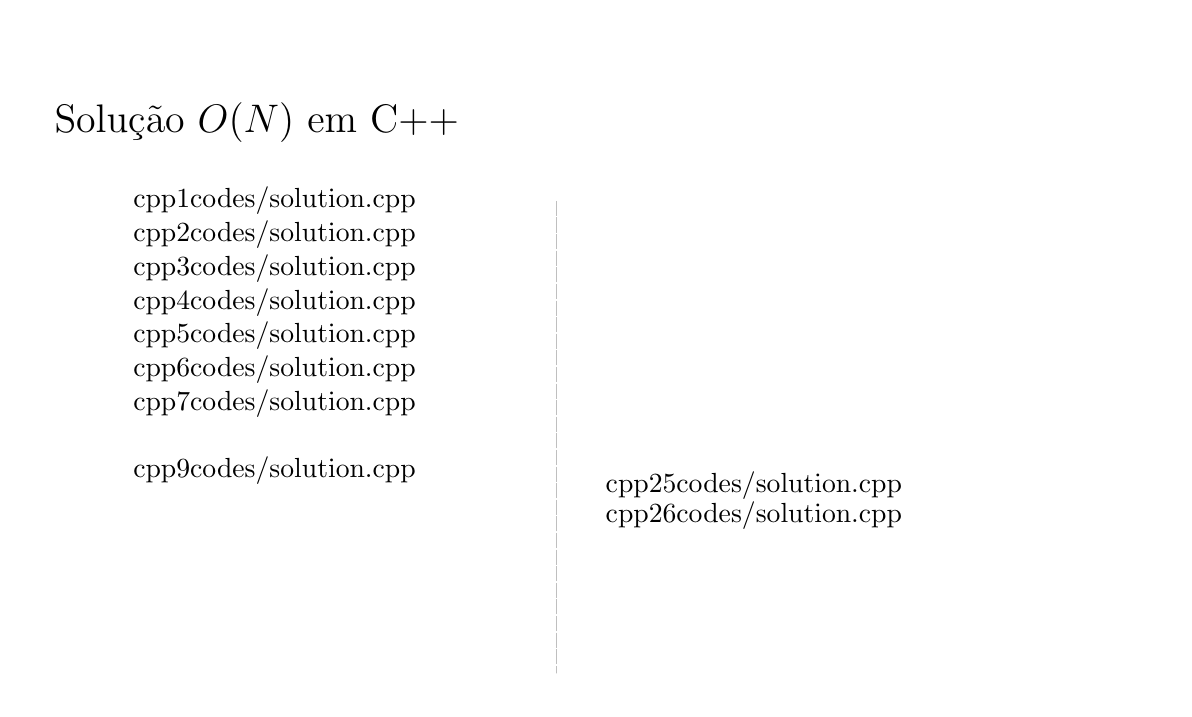
\begin{tikzpicture}
\node[draw,opacity=0] at (0, 0) {x};
\node[draw,opacity=0] at (14, 8) {x};

	\node[anchor=west] (title) at (0.0, 7.0) { \Large \bbbold{Solução $O(N)$ em C++} };

	\node[anchor=west] (line1) at (1.0, 6.0) { \inputline{cpp}{1}{codes/solution.cpp} };

	\node[anchor=west] (line2) at (1.0, 5.57) { \inputline{cpp}{2}{codes/solution.cpp} };

	\node[anchor=west] (line3) at (1.0, 5.14) { \inputline{cpp}{3}{codes/solution.cpp} };

	\node[anchor=west] (line4) at (1.0, 4.71) { \inputline{cpp}{4}{codes/solution.cpp} };

	\node[anchor=west] (line5) at (1.0, 4.29) { \inputline{cpp}{5}{codes/solution.cpp} };

	\node[anchor=west] (line6) at (1.0, 3.86) { \inputline{cpp}{6}{codes/solution.cpp} };

	\node[anchor=west] (line7) at (1.0, 3.43) { \inputline{cpp}{7}{codes/solution.cpp} };


	\node[anchor=west] (line9) at (1.0, 2.57) { \inputline{cpp}{9}{codes/solution.cpp} };















	\node[anchor=west] (line25) at (7.0, 2.39) { \inputline{cpp}{25}{codes/solution.cpp} };

	\node[anchor=west] (line26) at (7.0, 2.0) { \inputline{cpp}{26}{codes/solution.cpp} };

	\draw[color=gray!50,dashed] (6.5, 6) -- (6.5, 0) -- cycle;



\end{tikzpicture}
\end{frame}
\begin{frame}[plain,t]
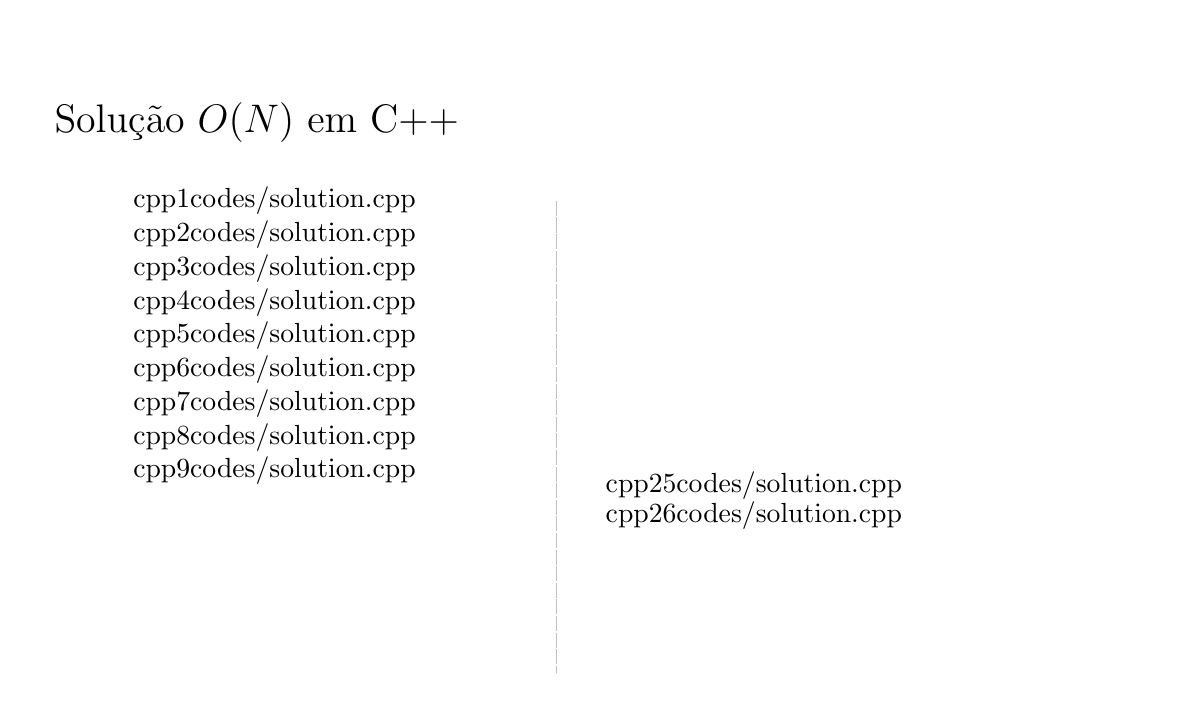
\begin{tikzpicture}
\node[draw,opacity=0] at (0, 0) {x};
\node[draw,opacity=0] at (14, 8) {x};

	\node[anchor=west] (title) at (0.0, 7.0) { \Large \bbbold{Solução $O(N)$ em C++} };

	\node[anchor=west] (line1) at (1.0, 6.0) { \inputline{cpp}{1}{codes/solution.cpp} };

	\node[anchor=west] (line2) at (1.0, 5.57) { \inputline{cpp}{2}{codes/solution.cpp} };

	\node[anchor=west] (line3) at (1.0, 5.14) { \inputline{cpp}{3}{codes/solution.cpp} };

	\node[anchor=west] (line4) at (1.0, 4.71) { \inputline{cpp}{4}{codes/solution.cpp} };

	\node[anchor=west] (line5) at (1.0, 4.29) { \inputline{cpp}{5}{codes/solution.cpp} };

	\node[anchor=west] (line6) at (1.0, 3.86) { \inputline{cpp}{6}{codes/solution.cpp} };

	\node[anchor=west] (line7) at (1.0, 3.43) { \inputline{cpp}{7}{codes/solution.cpp} };

	\node[anchor=west] (line8) at (1.0, 3.0) { \inputline{cpp}{8}{codes/solution.cpp} };

	\node[anchor=west] (line9) at (1.0, 2.57) { \inputline{cpp}{9}{codes/solution.cpp} };















	\node[anchor=west] (line25) at (7.0, 2.39) { \inputline{cpp}{25}{codes/solution.cpp} };

	\node[anchor=west] (line26) at (7.0, 2.0) { \inputline{cpp}{26}{codes/solution.cpp} };

	\draw[color=gray!50,dashed] (6.5, 6) -- (6.5, 0) -- cycle;




\end{tikzpicture}
\end{frame}
\begin{frame}[plain,t]
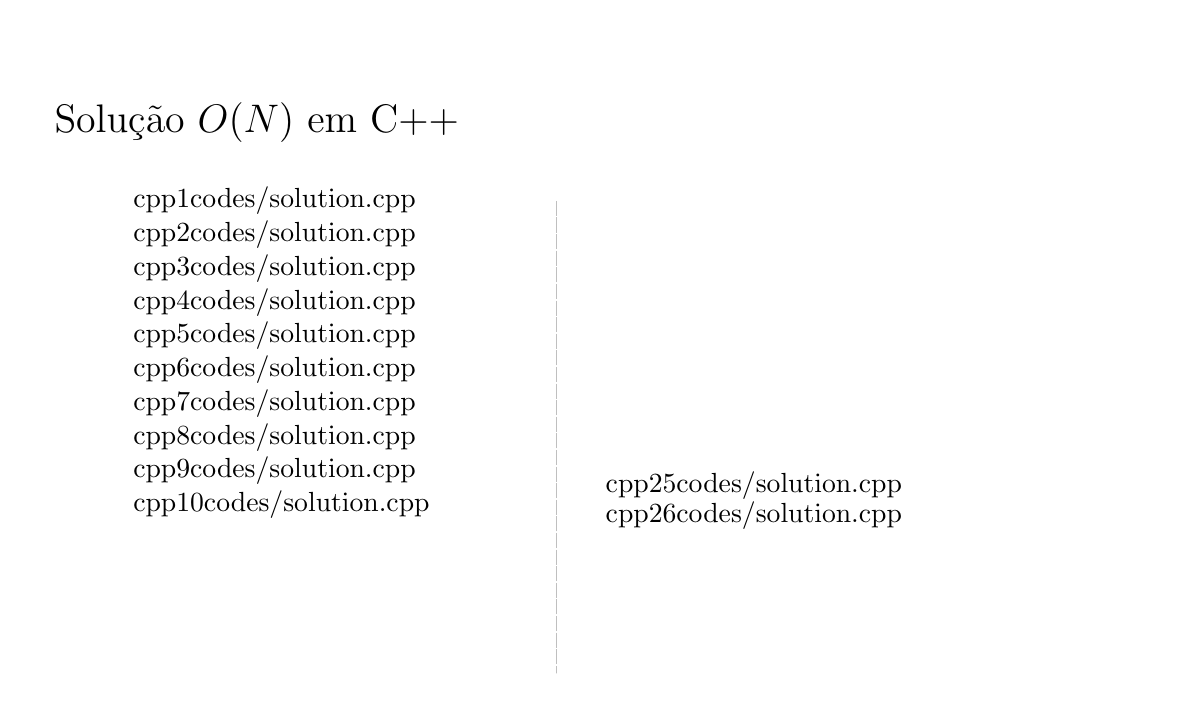
\begin{tikzpicture}
\node[draw,opacity=0] at (0, 0) {x};
\node[draw,opacity=0] at (14, 8) {x};

	\node[anchor=west] (title) at (0.0, 7.0) { \Large \bbbold{Solução $O(N)$ em C++} };

	\node[anchor=west] (line1) at (1.0, 6.0) { \inputline{cpp}{1}{codes/solution.cpp} };

	\node[anchor=west] (line2) at (1.0, 5.57) { \inputline{cpp}{2}{codes/solution.cpp} };

	\node[anchor=west] (line3) at (1.0, 5.14) { \inputline{cpp}{3}{codes/solution.cpp} };

	\node[anchor=west] (line4) at (1.0, 4.71) { \inputline{cpp}{4}{codes/solution.cpp} };

	\node[anchor=west] (line5) at (1.0, 4.29) { \inputline{cpp}{5}{codes/solution.cpp} };

	\node[anchor=west] (line6) at (1.0, 3.86) { \inputline{cpp}{6}{codes/solution.cpp} };

	\node[anchor=west] (line7) at (1.0, 3.43) { \inputline{cpp}{7}{codes/solution.cpp} };

	\node[anchor=west] (line8) at (1.0, 3.0) { \inputline{cpp}{8}{codes/solution.cpp} };

	\node[anchor=west] (line9) at (1.0, 2.57) { \inputline{cpp}{9}{codes/solution.cpp} };

	\node[anchor=west] (line10) at (1.0, 2.14) { \inputline{cpp}{10}{codes/solution.cpp} };














	\node[anchor=west] (line25) at (7.0, 2.39) { \inputline{cpp}{25}{codes/solution.cpp} };

	\node[anchor=west] (line26) at (7.0, 2.0) { \inputline{cpp}{26}{codes/solution.cpp} };

	\draw[color=gray!50,dashed] (6.5, 6) -- (6.5, 0) -- cycle;





\end{tikzpicture}
\end{frame}
\begin{frame}[plain,t]
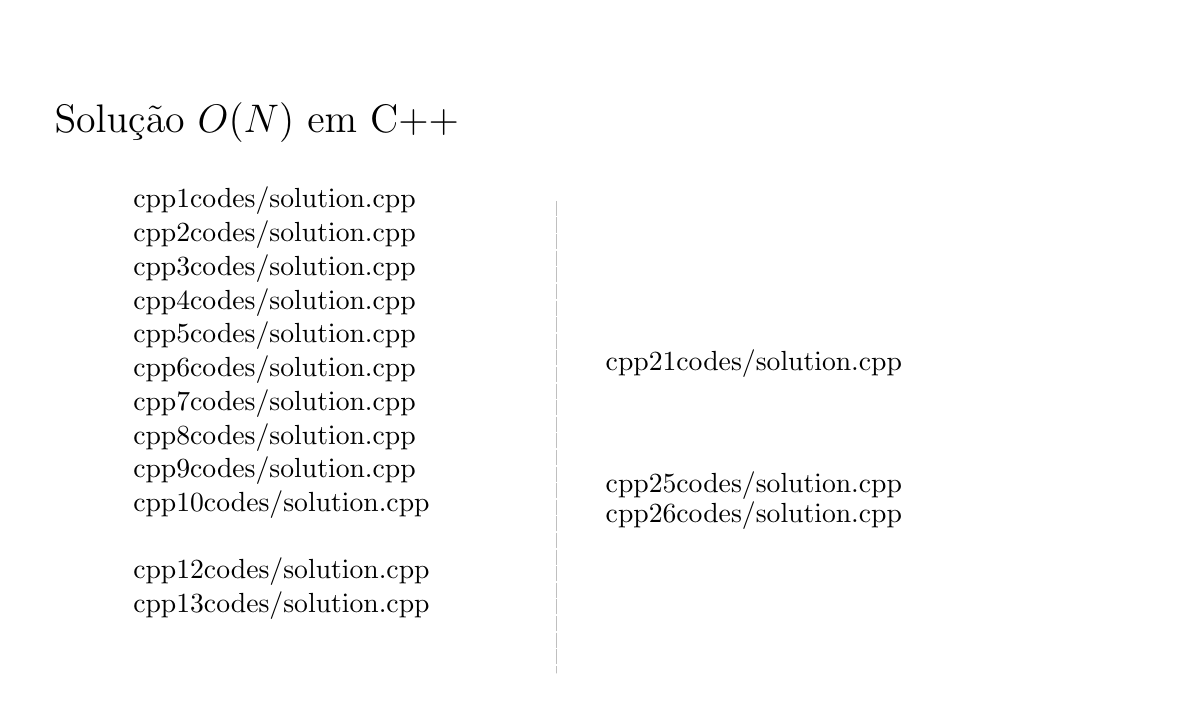
\begin{tikzpicture}
\node[draw,opacity=0] at (0, 0) {x};
\node[draw,opacity=0] at (14, 8) {x};

	\node[anchor=west] (title) at (0.0, 7.0) { \Large \bbbold{Solução $O(N)$ em C++} };

	\node[anchor=west] (line1) at (1.0, 6.0) { \inputline{cpp}{1}{codes/solution.cpp} };

	\node[anchor=west] (line2) at (1.0, 5.57) { \inputline{cpp}{2}{codes/solution.cpp} };

	\node[anchor=west] (line3) at (1.0, 5.14) { \inputline{cpp}{3}{codes/solution.cpp} };

	\node[anchor=west] (line4) at (1.0, 4.71) { \inputline{cpp}{4}{codes/solution.cpp} };

	\node[anchor=west] (line5) at (1.0, 4.29) { \inputline{cpp}{5}{codes/solution.cpp} };

	\node[anchor=west] (line6) at (1.0, 3.86) { \inputline{cpp}{6}{codes/solution.cpp} };

	\node[anchor=west] (line7) at (1.0, 3.43) { \inputline{cpp}{7}{codes/solution.cpp} };

	\node[anchor=west] (line8) at (1.0, 3.0) { \inputline{cpp}{8}{codes/solution.cpp} };

	\node[anchor=west] (line9) at (1.0, 2.57) { \inputline{cpp}{9}{codes/solution.cpp} };

	\node[anchor=west] (line10) at (1.0, 2.14) { \inputline{cpp}{10}{codes/solution.cpp} };


	\node[anchor=west] (line12) at (1.0, 1.29) { \inputline{cpp}{12}{codes/solution.cpp} };

	\node[anchor=west] (line13) at (1.0, 0.86) { \inputline{cpp}{13}{codes/solution.cpp} };







	\node[anchor=west] (line21) at (7.0, 3.94) { \inputline{cpp}{21}{codes/solution.cpp} };




	\node[anchor=west] (line25) at (7.0, 2.39) { \inputline{cpp}{25}{codes/solution.cpp} };

	\node[anchor=west] (line26) at (7.0, 2.0) { \inputline{cpp}{26}{codes/solution.cpp} };

	\draw[color=gray!50,dashed] (6.5, 6) -- (6.5, 0) -- cycle;






\end{tikzpicture}
\end{frame}
\begin{frame}[plain,t]
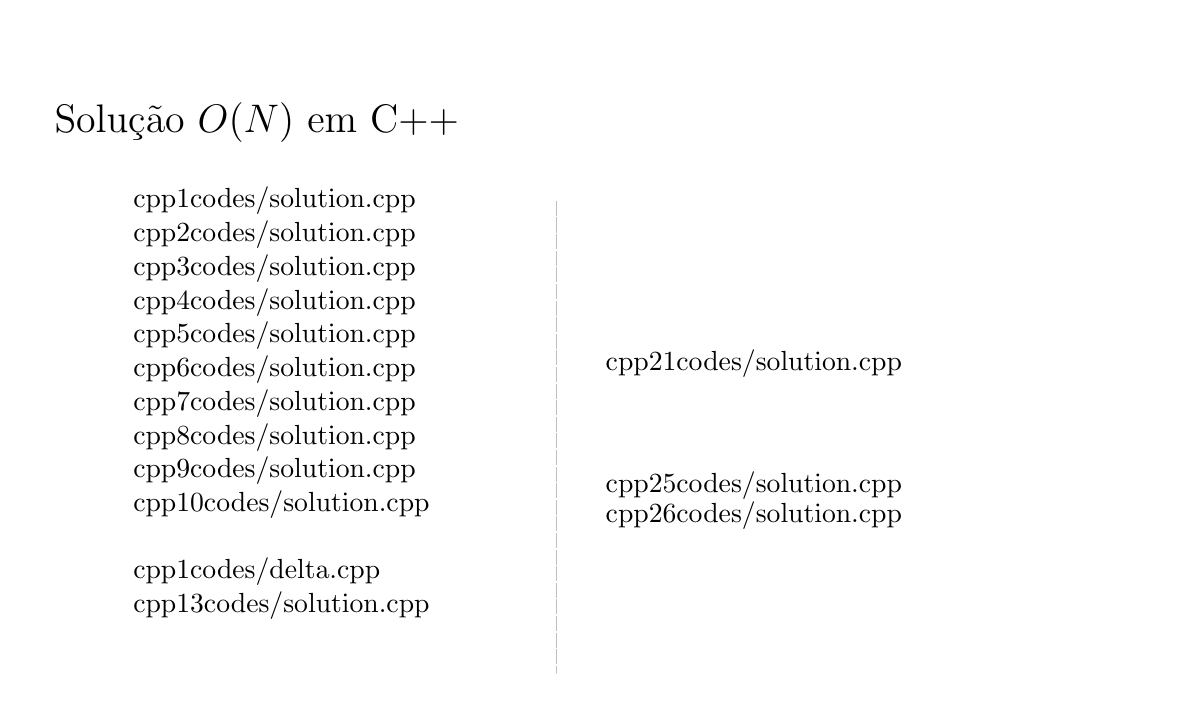
\begin{tikzpicture}
\node[draw,opacity=0] at (0, 0) {x};
\node[draw,opacity=0] at (14, 8) {x};

	\node[anchor=west] (title) at (0.0, 7.0) { \Large \bbbold{Solução $O(N)$ em C++} };

	\node[anchor=west] (line1) at (1.0, 6.0) { \inputline{cpp}{1}{codes/solution.cpp} };

	\node[anchor=west] (line2) at (1.0, 5.57) { \inputline{cpp}{2}{codes/solution.cpp} };

	\node[anchor=west] (line3) at (1.0, 5.14) { \inputline{cpp}{3}{codes/solution.cpp} };

	\node[anchor=west] (line4) at (1.0, 4.71) { \inputline{cpp}{4}{codes/solution.cpp} };

	\node[anchor=west] (line5) at (1.0, 4.29) { \inputline{cpp}{5}{codes/solution.cpp} };

	\node[anchor=west] (line6) at (1.0, 3.86) { \inputline{cpp}{6}{codes/solution.cpp} };

	\node[anchor=west] (line7) at (1.0, 3.43) { \inputline{cpp}{7}{codes/solution.cpp} };

	\node[anchor=west] (line8) at (1.0, 3.0) { \inputline{cpp}{8}{codes/solution.cpp} };

	\node[anchor=west] (line9) at (1.0, 2.57) { \inputline{cpp}{9}{codes/solution.cpp} };

	\node[anchor=west] (line10) at (1.0, 2.14) { \inputline{cpp}{10}{codes/solution.cpp} };


	\node[anchor=west] (line12) at (1.0, 1.29) { \inputline{cpp}{1}{codes/delta.cpp} };

	\node[anchor=west] (line13) at (1.0, 0.86) { \inputline{cpp}{13}{codes/solution.cpp} };







	\node[anchor=west] (line21) at (7.0, 3.94) { \inputline{cpp}{21}{codes/solution.cpp} };




	\node[anchor=west] (line25) at (7.0, 2.39) { \inputline{cpp}{25}{codes/solution.cpp} };

	\node[anchor=west] (line26) at (7.0, 2.0) { \inputline{cpp}{26}{codes/solution.cpp} };

	\draw[color=gray!50,dashed] (6.5, 6) -- (6.5, 0) -- cycle;








\end{tikzpicture}
\end{frame}
\begin{frame}[plain,t]
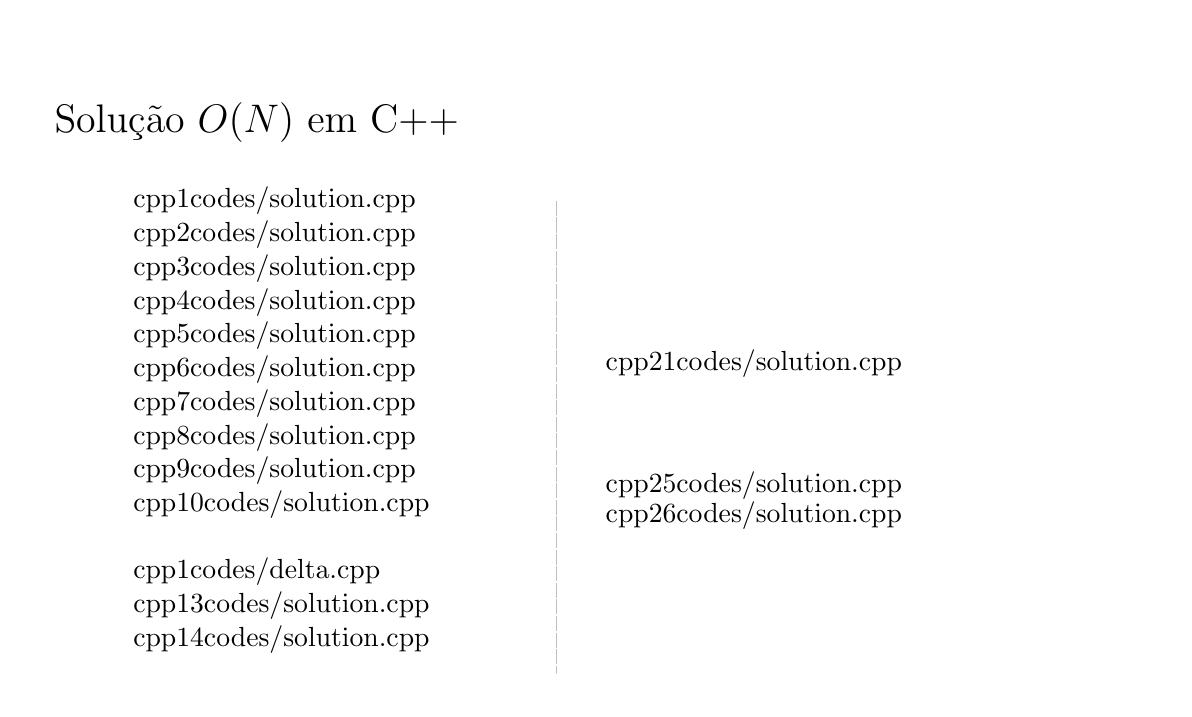
\begin{tikzpicture}
\node[draw,opacity=0] at (0, 0) {x};
\node[draw,opacity=0] at (14, 8) {x};

	\node[anchor=west] (title) at (0.0, 7.0) { \Large \bbbold{Solução $O(N)$ em C++} };

	\node[anchor=west] (line1) at (1.0, 6.0) { \inputline{cpp}{1}{codes/solution.cpp} };

	\node[anchor=west] (line2) at (1.0, 5.57) { \inputline{cpp}{2}{codes/solution.cpp} };

	\node[anchor=west] (line3) at (1.0, 5.14) { \inputline{cpp}{3}{codes/solution.cpp} };

	\node[anchor=west] (line4) at (1.0, 4.71) { \inputline{cpp}{4}{codes/solution.cpp} };

	\node[anchor=west] (line5) at (1.0, 4.29) { \inputline{cpp}{5}{codes/solution.cpp} };

	\node[anchor=west] (line6) at (1.0, 3.86) { \inputline{cpp}{6}{codes/solution.cpp} };

	\node[anchor=west] (line7) at (1.0, 3.43) { \inputline{cpp}{7}{codes/solution.cpp} };

	\node[anchor=west] (line8) at (1.0, 3.0) { \inputline{cpp}{8}{codes/solution.cpp} };

	\node[anchor=west] (line9) at (1.0, 2.57) { \inputline{cpp}{9}{codes/solution.cpp} };

	\node[anchor=west] (line10) at (1.0, 2.14) { \inputline{cpp}{10}{codes/solution.cpp} };


	\node[anchor=west] (line12) at (1.0, 1.29) { \inputline{cpp}{1}{codes/delta.cpp} };

	\node[anchor=west] (line13) at (1.0, 0.86) { \inputline{cpp}{13}{codes/solution.cpp} };

	\node[anchor=west] (line14) at (1.0, 0.43) { \inputline{cpp}{14}{codes/solution.cpp} };






	\node[anchor=west] (line21) at (7.0, 3.94) { \inputline{cpp}{21}{codes/solution.cpp} };




	\node[anchor=west] (line25) at (7.0, 2.39) { \inputline{cpp}{25}{codes/solution.cpp} };

	\node[anchor=west] (line26) at (7.0, 2.0) { \inputline{cpp}{26}{codes/solution.cpp} };

	\draw[color=gray!50,dashed] (6.5, 6) -- (6.5, 0) -- cycle;









\end{tikzpicture}
\end{frame}
\begin{frame}[plain,t]
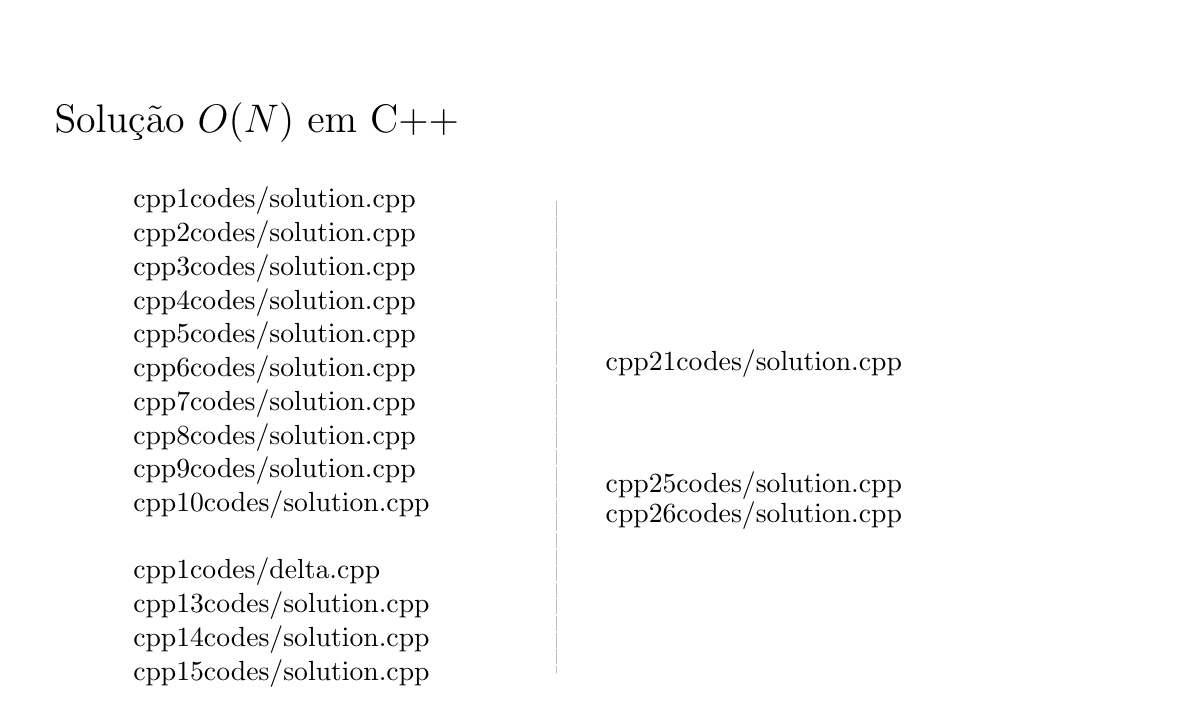
\begin{tikzpicture}
\node[draw,opacity=0] at (0, 0) {x};
\node[draw,opacity=0] at (14, 8) {x};

	\node[anchor=west] (title) at (0.0, 7.0) { \Large \bbbold{Solução $O(N)$ em C++} };

	\node[anchor=west] (line1) at (1.0, 6.0) { \inputline{cpp}{1}{codes/solution.cpp} };

	\node[anchor=west] (line2) at (1.0, 5.57) { \inputline{cpp}{2}{codes/solution.cpp} };

	\node[anchor=west] (line3) at (1.0, 5.14) { \inputline{cpp}{3}{codes/solution.cpp} };

	\node[anchor=west] (line4) at (1.0, 4.71) { \inputline{cpp}{4}{codes/solution.cpp} };

	\node[anchor=west] (line5) at (1.0, 4.29) { \inputline{cpp}{5}{codes/solution.cpp} };

	\node[anchor=west] (line6) at (1.0, 3.86) { \inputline{cpp}{6}{codes/solution.cpp} };

	\node[anchor=west] (line7) at (1.0, 3.43) { \inputline{cpp}{7}{codes/solution.cpp} };

	\node[anchor=west] (line8) at (1.0, 3.0) { \inputline{cpp}{8}{codes/solution.cpp} };

	\node[anchor=west] (line9) at (1.0, 2.57) { \inputline{cpp}{9}{codes/solution.cpp} };

	\node[anchor=west] (line10) at (1.0, 2.14) { \inputline{cpp}{10}{codes/solution.cpp} };


	\node[anchor=west] (line12) at (1.0, 1.29) { \inputline{cpp}{1}{codes/delta.cpp} };

	\node[anchor=west] (line13) at (1.0, 0.86) { \inputline{cpp}{13}{codes/solution.cpp} };

	\node[anchor=west] (line14) at (1.0, 0.43) { \inputline{cpp}{14}{codes/solution.cpp} };

	\node[anchor=west] (line15) at (1.0, -0.0) { \inputline{cpp}{15}{codes/solution.cpp} };





	\node[anchor=west] (line21) at (7.0, 3.94) { \inputline{cpp}{21}{codes/solution.cpp} };




	\node[anchor=west] (line25) at (7.0, 2.39) { \inputline{cpp}{25}{codes/solution.cpp} };

	\node[anchor=west] (line26) at (7.0, 2.0) { \inputline{cpp}{26}{codes/solution.cpp} };

	\draw[color=gray!50,dashed] (6.5, 6) -- (6.5, 0) -- cycle;










\end{tikzpicture}
\end{frame}
\begin{frame}[plain,t]
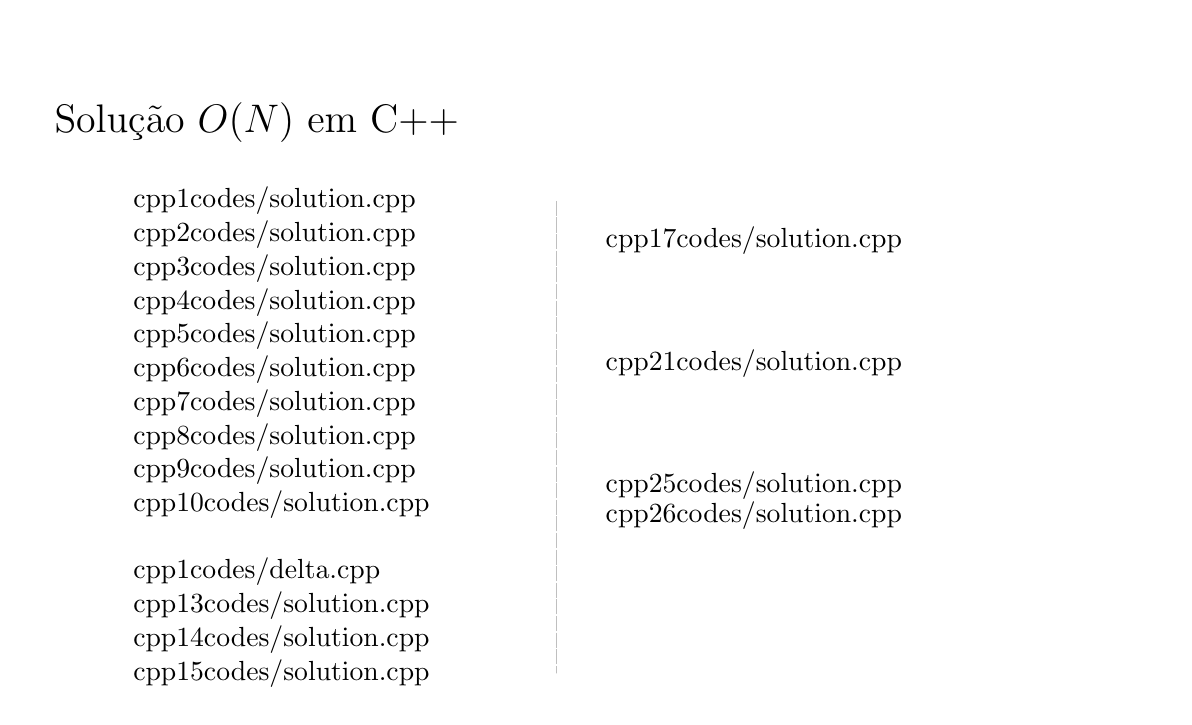
\begin{tikzpicture}
\node[draw,opacity=0] at (0, 0) {x};
\node[draw,opacity=0] at (14, 8) {x};

	\node[anchor=west] (title) at (0.0, 7.0) { \Large \bbbold{Solução $O(N)$ em C++} };

	\node[anchor=west] (line1) at (1.0, 6.0) { \inputline{cpp}{1}{codes/solution.cpp} };

	\node[anchor=west] (line2) at (1.0, 5.57) { \inputline{cpp}{2}{codes/solution.cpp} };

	\node[anchor=west] (line3) at (1.0, 5.14) { \inputline{cpp}{3}{codes/solution.cpp} };

	\node[anchor=west] (line4) at (1.0, 4.71) { \inputline{cpp}{4}{codes/solution.cpp} };

	\node[anchor=west] (line5) at (1.0, 4.29) { \inputline{cpp}{5}{codes/solution.cpp} };

	\node[anchor=west] (line6) at (1.0, 3.86) { \inputline{cpp}{6}{codes/solution.cpp} };

	\node[anchor=west] (line7) at (1.0, 3.43) { \inputline{cpp}{7}{codes/solution.cpp} };

	\node[anchor=west] (line8) at (1.0, 3.0) { \inputline{cpp}{8}{codes/solution.cpp} };

	\node[anchor=west] (line9) at (1.0, 2.57) { \inputline{cpp}{9}{codes/solution.cpp} };

	\node[anchor=west] (line10) at (1.0, 2.14) { \inputline{cpp}{10}{codes/solution.cpp} };


	\node[anchor=west] (line12) at (1.0, 1.29) { \inputline{cpp}{1}{codes/delta.cpp} };

	\node[anchor=west] (line13) at (1.0, 0.86) { \inputline{cpp}{13}{codes/solution.cpp} };

	\node[anchor=west] (line14) at (1.0, 0.43) { \inputline{cpp}{14}{codes/solution.cpp} };

	\node[anchor=west] (line15) at (1.0, -0.0) { \inputline{cpp}{15}{codes/solution.cpp} };

	\node[anchor=west] (line17) at (7.0, 5.5) { \inputline{cpp}{17}{codes/solution.cpp} };




	\node[anchor=west] (line21) at (7.0, 3.94) { \inputline{cpp}{21}{codes/solution.cpp} };




	\node[anchor=west] (line25) at (7.0, 2.39) { \inputline{cpp}{25}{codes/solution.cpp} };

	\node[anchor=west] (line26) at (7.0, 2.0) { \inputline{cpp}{26}{codes/solution.cpp} };

	\draw[color=gray!50,dashed] (6.5, 6) -- (6.5, 0) -- cycle;











\end{tikzpicture}
\end{frame}
\begin{frame}[plain,t]
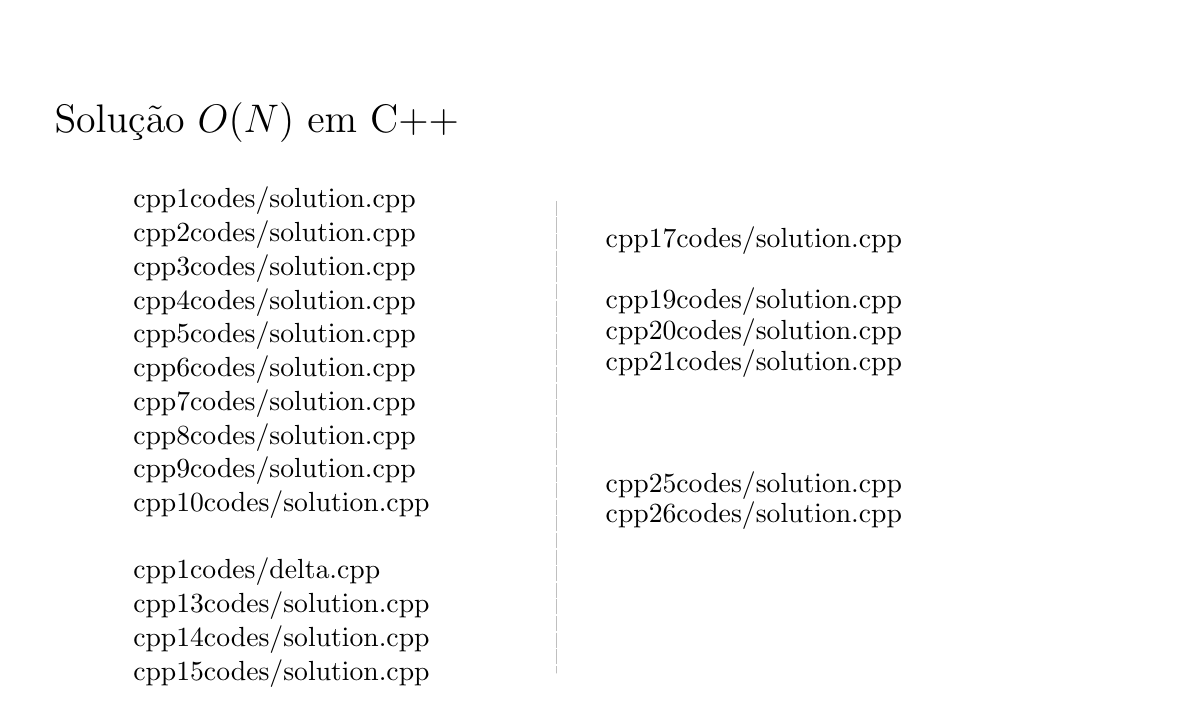
\begin{tikzpicture}
\node[draw,opacity=0] at (0, 0) {x};
\node[draw,opacity=0] at (14, 8) {x};

	\node[anchor=west] (title) at (0.0, 7.0) { \Large \bbbold{Solução $O(N)$ em C++} };

	\node[anchor=west] (line1) at (1.0, 6.0) { \inputline{cpp}{1}{codes/solution.cpp} };

	\node[anchor=west] (line2) at (1.0, 5.57) { \inputline{cpp}{2}{codes/solution.cpp} };

	\node[anchor=west] (line3) at (1.0, 5.14) { \inputline{cpp}{3}{codes/solution.cpp} };

	\node[anchor=west] (line4) at (1.0, 4.71) { \inputline{cpp}{4}{codes/solution.cpp} };

	\node[anchor=west] (line5) at (1.0, 4.29) { \inputline{cpp}{5}{codes/solution.cpp} };

	\node[anchor=west] (line6) at (1.0, 3.86) { \inputline{cpp}{6}{codes/solution.cpp} };

	\node[anchor=west] (line7) at (1.0, 3.43) { \inputline{cpp}{7}{codes/solution.cpp} };

	\node[anchor=west] (line8) at (1.0, 3.0) { \inputline{cpp}{8}{codes/solution.cpp} };

	\node[anchor=west] (line9) at (1.0, 2.57) { \inputline{cpp}{9}{codes/solution.cpp} };

	\node[anchor=west] (line10) at (1.0, 2.14) { \inputline{cpp}{10}{codes/solution.cpp} };


	\node[anchor=west] (line12) at (1.0, 1.29) { \inputline{cpp}{1}{codes/delta.cpp} };

	\node[anchor=west] (line13) at (1.0, 0.86) { \inputline{cpp}{13}{codes/solution.cpp} };

	\node[anchor=west] (line14) at (1.0, 0.43) { \inputline{cpp}{14}{codes/solution.cpp} };

	\node[anchor=west] (line15) at (1.0, -0.0) { \inputline{cpp}{15}{codes/solution.cpp} };

	\node[anchor=west] (line17) at (7.0, 5.5) { \inputline{cpp}{17}{codes/solution.cpp} };


	\node[anchor=west] (line19) at (7.0, 4.72) { \inputline{cpp}{19}{codes/solution.cpp} };

	\node[anchor=west] (line20) at (7.0, 4.33) { \inputline{cpp}{20}{codes/solution.cpp} };

	\node[anchor=west] (line21) at (7.0, 3.94) { \inputline{cpp}{21}{codes/solution.cpp} };




	\node[anchor=west] (line25) at (7.0, 2.39) { \inputline{cpp}{25}{codes/solution.cpp} };

	\node[anchor=west] (line26) at (7.0, 2.0) { \inputline{cpp}{26}{codes/solution.cpp} };

	\draw[color=gray!50,dashed] (6.5, 6) -- (6.5, 0) -- cycle;












\end{tikzpicture}
\end{frame}
\begin{frame}[plain,t]
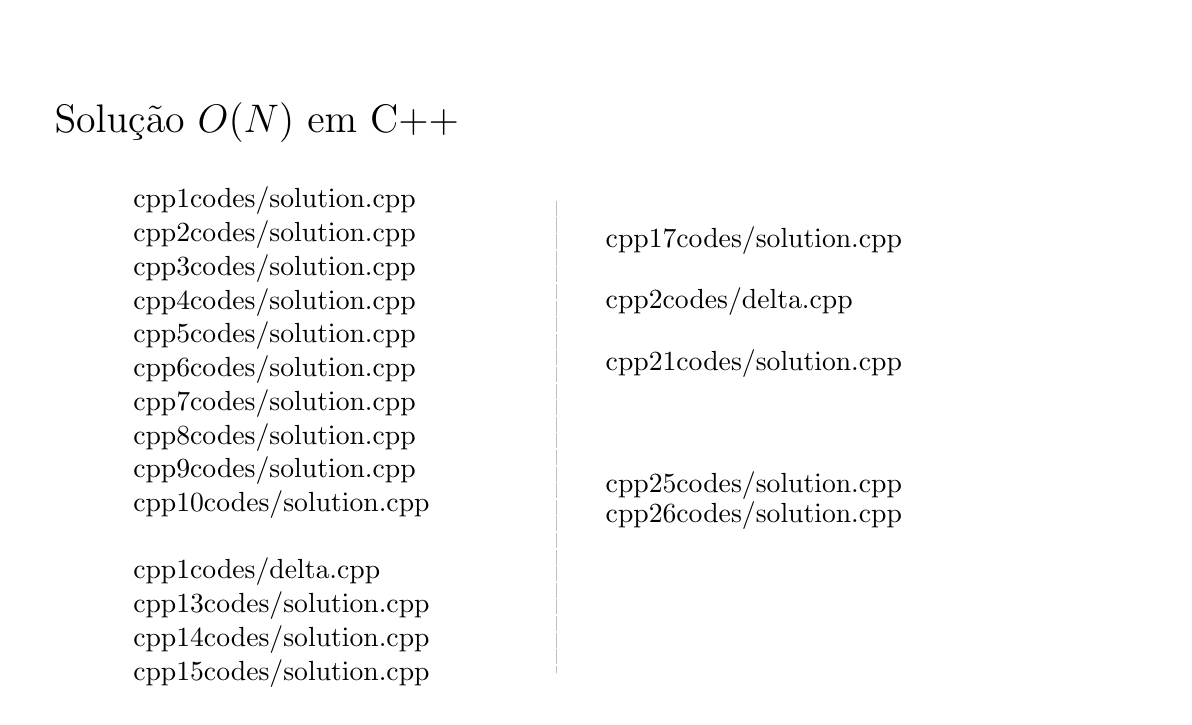
\begin{tikzpicture}
\node[draw,opacity=0] at (0, 0) {x};
\node[draw,opacity=0] at (14, 8) {x};

	\node[anchor=west] (title) at (0.0, 7.0) { \Large \bbbold{Solução $O(N)$ em C++} };

	\node[anchor=west] (line1) at (1.0, 6.0) { \inputline{cpp}{1}{codes/solution.cpp} };

	\node[anchor=west] (line2) at (1.0, 5.57) { \inputline{cpp}{2}{codes/solution.cpp} };

	\node[anchor=west] (line3) at (1.0, 5.14) { \inputline{cpp}{3}{codes/solution.cpp} };

	\node[anchor=west] (line4) at (1.0, 4.71) { \inputline{cpp}{4}{codes/solution.cpp} };

	\node[anchor=west] (line5) at (1.0, 4.29) { \inputline{cpp}{5}{codes/solution.cpp} };

	\node[anchor=west] (line6) at (1.0, 3.86) { \inputline{cpp}{6}{codes/solution.cpp} };

	\node[anchor=west] (line7) at (1.0, 3.43) { \inputline{cpp}{7}{codes/solution.cpp} };

	\node[anchor=west] (line8) at (1.0, 3.0) { \inputline{cpp}{8}{codes/solution.cpp} };

	\node[anchor=west] (line9) at (1.0, 2.57) { \inputline{cpp}{9}{codes/solution.cpp} };

	\node[anchor=west] (line10) at (1.0, 2.14) { \inputline{cpp}{10}{codes/solution.cpp} };


	\node[anchor=west] (line12) at (1.0, 1.29) { \inputline{cpp}{1}{codes/delta.cpp} };

	\node[anchor=west] (line13) at (1.0, 0.86) { \inputline{cpp}{13}{codes/solution.cpp} };

	\node[anchor=west] (line14) at (1.0, 0.43) { \inputline{cpp}{14}{codes/solution.cpp} };

	\node[anchor=west] (line15) at (1.0, -0.0) { \inputline{cpp}{15}{codes/solution.cpp} };

	\node[anchor=west] (line17) at (7.0, 5.5) { \inputline{cpp}{17}{codes/solution.cpp} };


	\node[anchor=west] (line19) at (7.0, 4.72) { \inputline{cpp}{2}{codes/delta.cpp} };


	\node[anchor=west] (line21) at (7.0, 3.94) { \inputline{cpp}{21}{codes/solution.cpp} };




	\node[anchor=west] (line25) at (7.0, 2.39) { \inputline{cpp}{25}{codes/solution.cpp} };

	\node[anchor=west] (line26) at (7.0, 2.0) { \inputline{cpp}{26}{codes/solution.cpp} };

	\draw[color=gray!50,dashed] (6.5, 6) -- (6.5, 0) -- cycle;













\end{tikzpicture}
\end{frame}
\begin{frame}[plain,t]
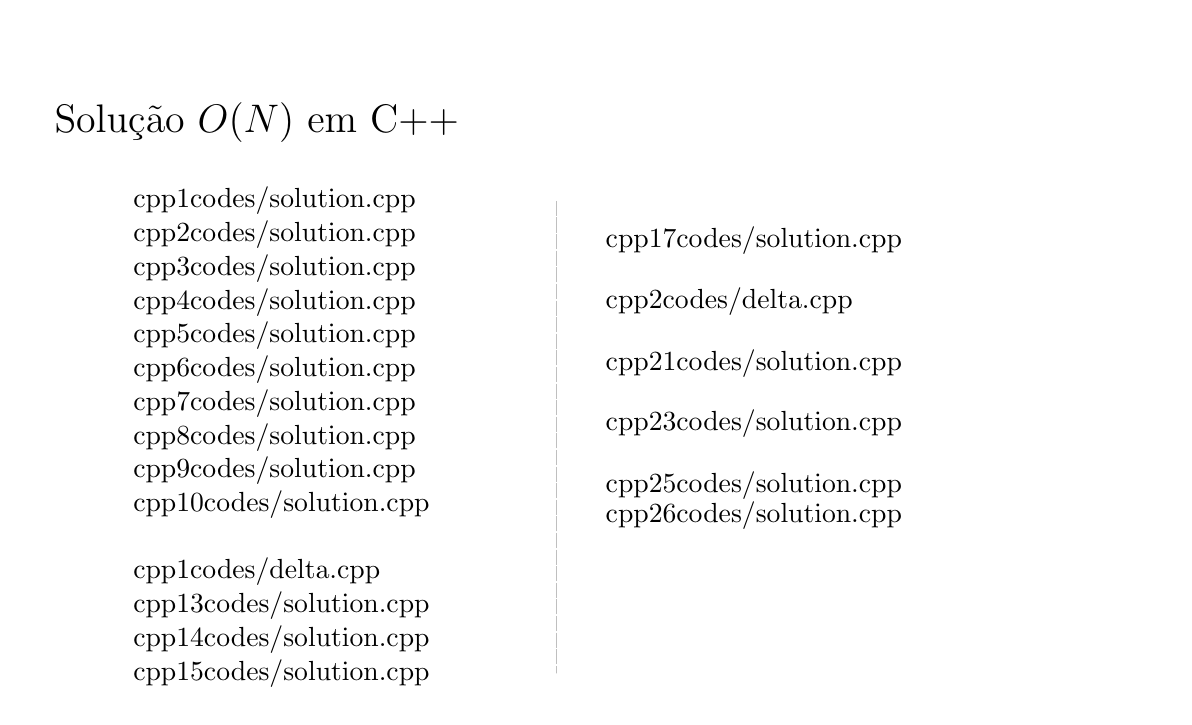
\begin{tikzpicture}
\node[draw,opacity=0] at (0, 0) {x};
\node[draw,opacity=0] at (14, 8) {x};

	\node[anchor=west] (title) at (0.0, 7.0) { \Large \bbbold{Solução $O(N)$ em C++} };

	\node[anchor=west] (line1) at (1.0, 6.0) { \inputline{cpp}{1}{codes/solution.cpp} };

	\node[anchor=west] (line2) at (1.0, 5.57) { \inputline{cpp}{2}{codes/solution.cpp} };

	\node[anchor=west] (line3) at (1.0, 5.14) { \inputline{cpp}{3}{codes/solution.cpp} };

	\node[anchor=west] (line4) at (1.0, 4.71) { \inputline{cpp}{4}{codes/solution.cpp} };

	\node[anchor=west] (line5) at (1.0, 4.29) { \inputline{cpp}{5}{codes/solution.cpp} };

	\node[anchor=west] (line6) at (1.0, 3.86) { \inputline{cpp}{6}{codes/solution.cpp} };

	\node[anchor=west] (line7) at (1.0, 3.43) { \inputline{cpp}{7}{codes/solution.cpp} };

	\node[anchor=west] (line8) at (1.0, 3.0) { \inputline{cpp}{8}{codes/solution.cpp} };

	\node[anchor=west] (line9) at (1.0, 2.57) { \inputline{cpp}{9}{codes/solution.cpp} };

	\node[anchor=west] (line10) at (1.0, 2.14) { \inputline{cpp}{10}{codes/solution.cpp} };


	\node[anchor=west] (line12) at (1.0, 1.29) { \inputline{cpp}{1}{codes/delta.cpp} };

	\node[anchor=west] (line13) at (1.0, 0.86) { \inputline{cpp}{13}{codes/solution.cpp} };

	\node[anchor=west] (line14) at (1.0, 0.43) { \inputline{cpp}{14}{codes/solution.cpp} };

	\node[anchor=west] (line15) at (1.0, -0.0) { \inputline{cpp}{15}{codes/solution.cpp} };

	\node[anchor=west] (line17) at (7.0, 5.5) { \inputline{cpp}{17}{codes/solution.cpp} };


	\node[anchor=west] (line19) at (7.0, 4.72) { \inputline{cpp}{2}{codes/delta.cpp} };


	\node[anchor=west] (line21) at (7.0, 3.94) { \inputline{cpp}{21}{codes/solution.cpp} };


	\node[anchor=west] (line23) at (7.0, 3.17) { \inputline{cpp}{23}{codes/solution.cpp} };


	\node[anchor=west] (line25) at (7.0, 2.39) { \inputline{cpp}{25}{codes/solution.cpp} };

	\node[anchor=west] (line26) at (7.0, 2.0) { \inputline{cpp}{26}{codes/solution.cpp} };

	\draw[color=gray!50,dashed] (6.5, 6) -- (6.5, 0) -- cycle;














\end{tikzpicture}
\end{frame}
\begin{frame}[plain,t]
\begin{tikzpicture}
\node[draw,opacity=0] at (0, 0) {x};
\node[draw,opacity=0] at (14, 8) {x};

	\node[anchor=west] (title) at (0.0, 6.0) { \Large \bbbold{Referências} };

	\node[anchor=west] (a) at (1.0, 4.5) { $\star$ \bbtext{Grandpa icon created by Freepik - Flaticon:} };

	\node[anchor=west] (a1) at (0.5, 4.0) { \url{https://www.flaticon.com/free-icons/grandpa} };



\end{tikzpicture}
\end{frame}
\end{document}
